\documentclass[]{beamer}
\usepackage{etex}
\usepackage{beamerthemesplit}
\usepackage{graphics,epsfig}
\usepackage{pstricks}
\usepackage{graphicx}
\usepackage{hyperref}
\usepackage{subfigure}
\usepackage{listings}
\usepackage{multirow}
\usepackage{xspace}
\usepackage[absolute,overlay]{textpos}
\setlength{\TPHorizModule}{1cm}
\setlength{\TPVertModule}{1cm}


\mode<presentation>
{ \usetheme{Boadilla}
  \setbeamercovered{transparent}
  \setbeamertemplate{items}[circle]
  \setbeamertemplate{theorems}[numbered]
  \setbeamertemplate{footline}[frame number]
}
 
%\useinnertheme[shadow=true]{rounded}
\useoutertheme{shadow}
\usecolortheme{whale}

\newcommand\blfootnote[1]{
  \begingroup
  \renewcommand\thefootnote{}\footnote{#1}
  \addtocounter{footnote}{-1}
  \endgroup
}


\mode
<all>

\title{C Programming}
\author{Wan-Lei Zhao}

\makeatletter
\makeatother

\begin{document}
\begin{frame}
   \begin{center}
    \vspace{24pt}
    \Huge\textbf{C Programming}\blfootnote{Email: wlzhao@xmu.edu.cn, copyrights are fully reserved by the author.}\\
     \Huge{Lecture 6: }\\
     \begin{figure}
     	\begin{center}
     		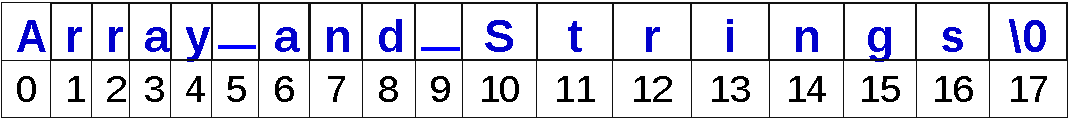
\includegraphics[width=0.75\linewidth]{figs/array_symb.pdf}
     	\end{center}
     \end{figure}
    \vspace{36pt}
  \end{center}
  \begin{align*}
   \vspace{18pt}
      \large{\mbox{Lecturer:}~Dr.~\mbox{Wan-Lei~~Zhao}} \\
      \large{Spring~~Semester~~2022} \\
   \vspace{30pt}
  \end{align*}
\end{frame}

\definecolor{cornblue}{HTML}{6495ED}
\definecolor{navyblue}{HTML}{000080}
\definecolor{midnblue}{HTML}{191970}
\definecolor{lghtblue}{HTML}{B0C4DE}
\setbeamercolor{background}{fg=black, bg=lghtblue}
\setbeamercolor{palette primary}{fg=white, bg=lghtblue}
\setbeamercolor{palette secondary}{fg=black, bg=cornblue}
\setbeamercolor{palette tertiary}{fg=black, bg=lghtblue}
\setbeamercolor{palette quaternary}{fg=black, bg=lghtblue}
\setbeamercolor{frametitle}{fg=black, bg=white}
\definecolor{ballblue}{rgb}{0.13, 0.67, 0.8}
\definecolor{cornflowerblue}{rgb}{0.39,0.58,0.93}
\definecolor{babyblueeyes}{rgb}{0.63, 0.79, 0.95}

\setbeamertemplate{footline}
{
  \leavevmode%
  \hbox{%
  \begin{beamercolorbox}[wd=.275\paperwidth,ht=2.25ex,dp=1ex,center]{author in head/foot}%
    \usebeamerfont{author in head/foot}\insertshortauthor
  \end{beamercolorbox}%
  \begin{beamercolorbox}[wd=.44\paperwidth,ht=2.25ex,dp=1ex,center]{title in head/foot}%
    \usebeamerfont{title in head/foot}\insertshorttitle\hspace*{3em}
    \hspace*{1ex}
  \end{beamercolorbox}%
  \begin{beamercolorbox}[wd=.285\paperwidth,ht=2.25ex,dp=1ex,center]{date/foot}%
    \usebeamerfont{title in head/foot}\hspace*{2em}
    \insertframenumber{} / \inserttotalframenumber\hspace*{1ex}
  \end{beamercolorbox}}%
  \vskip0pt
}



% preset-listing options
\lstset{
  backgroundcolor=\color{white},   
  basicstyle=\footnotesize,    
  language=c,
  breakatwhitespace=false,         
  breaklines=true,                 % sets automatic line breaking
  captionpos=b,                    % sets the caption-position to bottom
  commentstyle=\color{ballblue},    % comment style
  extendedchars=true,              
  frame=single,                    % adds a frame around the code     
  keywordstyle=\color{blue},       % keyword style
  numbers=left,                    
  numbersep=5pt,                   
  numberstyle=\tiny\color{blue}, 
  rulecolor=\color{babyblueeyes},
  stepnumber=1,              
  stringstyle=\color{black},     % string literal style
  tabsize=4,                       % sets default tabsize to 4 spaces
  title=\lstname                   
}


\section{Arrays}
\label{sec:arry}
\begin{frame}<beamer>
    \frametitle{Outline}
    \tableofcontents[currentsection]
\end{frame}

\begin{frame}[fragile]{Opening Discussion (1)}

\begin{itemize}
	\item {Given we have following problem}
	\begin{itemize}
		\item {We have 10 students in the class}
		\item {We want to get average/sum/max/min score of their math course}
		\item {We also want to rank the scores}
		\item {Based on what we learned}
		\item {We should keep 10 variables of the same type}
	\end{itemize}
	\item {How about we have 100 students??}
\end{itemize}
\vspace{-0.15in}
\begin{columns}
\begin{column}{0.75\linewidth}
\begin{lstlisting}
#include <stdio.h>
int main()
{
   float x1, x2, x3, x4, x5, x6,x7,x8,x9,x10;
   float sum = 0, avg = 0;
   scanf("%f", &x1);
   sum += x1;
   scanf("%f", &x2);
   sum += x2;
   ...
   avg = sum/10;
   return 0;
}
\end{lstlisting}
\end{column}
\end{columns}
\end{frame}

\begin{frame}[fragile]{Opening Discussion (2)}
\vspace{-0.15in}
\begin{columns}
\begin{column}{0.75\linewidth}
\begin{lstlisting}
#include <stdio.h>
int main()
{
   float x1, x2, x3, x4, x5, x6,x7,x8,x9,x10;
   float sum = 0, avg = 0;
   scanf("%f", &x1);
   sum += x1;
   scanf("%f", &x2);
   sum += x2;
   ...
   avg = sum/10;
   return 0;
}

\end{lstlisting}
\end{column}
\end{columns}
\vspace{-0.15in}
\begin{itemize}
	\item {Even that it is hard to do sorting}
	\begin{itemize}
		\item {Try your best to figure out how you can put fourty variables in order}
	\end{itemize}
	\item {This is where the \textcolor{red}{array} comes}
\end{itemize}

\end{frame}

\subsection{1D Array}
\label{sec:1darry}
\begin{frame}<beamer>
    \frametitle{Outline}
    \tableofcontents[currentsection, currentsubsection]
\end{frame}

\begin{frame}[fragile]{1D Array: declaration (1)}
\begin{itemize}
	\item {1D array is defined in following form}
\end{itemize}
\begin{center}
 \LARGE{
	\textcolor{blue}{type} \textcolor{red}{arrayName}[\textbf{size}];
	}
\end{center}
\begin{itemize}
	\item {\textcolor{blue}{type} could be any type defined in C, e.g. \textcolor{blue}{int}, \textcolor{blue}{float},...}
	\item {``\textcolor{red}{arrayName}'' should be \textcolor{red}{unique}}
	\item {It is actually a variable/constant, so rules to other variables/constants apply too}
	\item {``\textbf{size}'' should be an integer or an integer constant \textcolor{red}{greater than 0}}
\end{itemize}
\begin{lstlisting}[xleftmargin=0.09\linewidth, linewidth=0.9\linewidth, frame=no, numbers=none]
int a[0]; //it is grammar OK, but meaningless
\end{lstlisting}
\end{frame}

\begin{frame}[fragile]{1D Array: declaration (2)}
\begin{center}
 \LARGE{
	\textcolor{blue}{type} \textcolor{red}{arrayName}[\textbf{size}];
	}
\end{center}
\begin{itemize}
	\item {\textcolor{blue}{type} could be any type defined in C, e.g. \textcolor{blue}{int}, \textcolor{blue}{float},...}
	\item {``\textcolor{red}{arrayName}'' should be \textcolor{red}{unique}}
	\item {It is actually a variable/constant, so rules to other variables/constants apply too}
	\item {``\textbf{size}'' should be an integer or an integer constant \textcolor{red}{greater than 0}}
\end{itemize}
\begin{columns}
\begin{column}{0.25\linewidth}
\begin{lstlisting}
int main()
{
   float x[40];
   ....
   return 0;
}

\end{lstlisting}
\end{column}
\begin{column}{0.35\linewidth}
\begin{lstlisting}
int main()
{
   const int N = 40;
   float x[N];
   ....
   return 0;
}

\end{lstlisting}
\end{column}
\begin{column}{0.3\linewidth}
\begin{lstlisting}
int main()
{
   int N = 40;
   float x[N];
   ....
   return 0;
}

\end{lstlisting}
\end{column}
\end{columns}
\end{frame}

\begin{frame}[fragile]{1D Array: declaration (3)}
\begin{center}
 \LARGE{
	\textcolor{blue}{type} \textcolor{red}{arrayName}[\textbf{size}];
	}
\end{center}
\begin{itemize}
	\item {\textcolor{blue}{type} could be any type defined in C, e.g. \textcolor{blue}{int}, \textcolor{blue}{float},...}
	\item {``\textcolor{red}{arrayName}'' should be \textcolor{red}{unique}}
	\item {It is actually a variable/constant, so rules to other variables/constants apply too}
	\item {``\textbf{size}'' should be an integer or an integer constant \textcolor{red}{greater than 0}}
\end{itemize}
\begin{columns}
\begin{column}{0.25\linewidth}
\begin{lstlisting}
#define N 40
int main()
{
   float x[N];
   ....
   return 0;
}

\end{lstlisting}
\end{column}
\begin{column}{0.35\linewidth}
\begin{lstlisting}
int main()
{
   const int N = 40;
   float x[N];
   ....
   return 0;
}

\end{lstlisting}
\end{column}
\begin{column}{0.3\linewidth}
\begin{lstlisting}
#define N 40
int main()
{
   float x[3*N];
   ....
   return 0;
}

\end{lstlisting}
\end{column}
\end{columns}
\end{frame}

\begin{frame}[fragile]{1D Array: visit array element (1)}
\begin{itemize}
	\item {Element in an array is visited by the \textbf{subscript}}
	\item {Subscript starts from `\textcolor{green}{0}' to `\textcolor{green}{N-1}'}
	\item {For example, visit the 3rd element of x[N], we write ``x[2]''}
\end{itemize}
\begin{columns}
\begin{column}{0.2\linewidth}
\end{column}
\begin{column}{0.5\linewidth}
\begin{lstlisting}
#include <stdio.h>
int main()
{
   float x[40];
   x[0] = 5.0;
   x[2] = 3.1;
   printf("x[0] = %f", x[0]);
   return 0;
}

\end{lstlisting}
\end{column}
\begin{column}{0.2\linewidth}
\end{column}
\end{columns}
\end{frame}

\begin{frame}[fragile]{1D Array: visit array element (2)}
\begin{columns}
\begin{column}{0.2\linewidth}
\end{column}
\begin{column}{0.52\linewidth}
\begin{lstlisting}
int main()
{
   float x[40];
   int i = 0;
   for(i = 0; i < 40; i++)
   {
      printf("Input %d:", i);
      /*--be careful below--*/
      scanf("%f", &(x[i])); 
   }
   return 0;
}
\end{lstlisting}
\end{column}
\begin{column}{0.2\linewidth}
\end{column}
\end{columns}
\begin{itemize}
	\item {You are not allowed to use subscript beyond \textcolor{red}{39}}
	\item {You invade other's territory!!}
\end{itemize}
\end{frame}

\begin{frame}[fragile]{1D Array: how array looks like (1)}
\begin{columns}
\begin{column}{0.5\linewidth}
\begin{figure}
	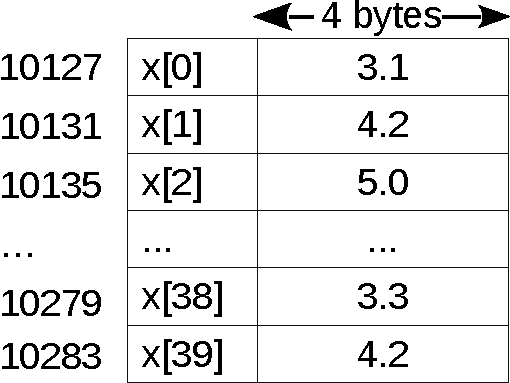
\includegraphics[width=0.88\linewidth]{figs/farray.pdf}
\end{figure}
\end{column}
\begin{column}{0.5\linewidth}
\begin{figure}
	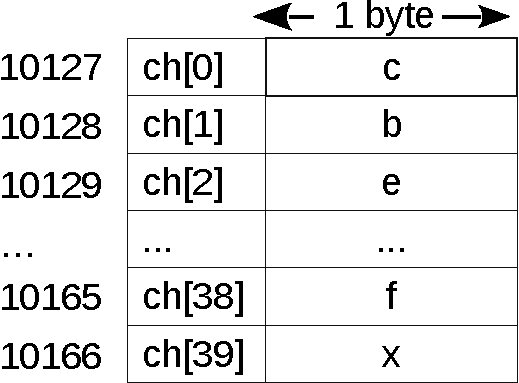
\includegraphics[width=0.9\linewidth]{figs/charray.pdf}
\end{figure}
\end{column}
\end{columns}
\vspace{0.1in}
\begin{itemize}
	\item {The system opens a continuous memory block for an array}
	\item {Actual size depends on both the type and length of an array}
\end{itemize}
\end{frame}

\begin{frame}[fragile]{1D Array: how array looks like (2)}
\begin{columns}
\begin{column}{0.46\linewidth}
\begin{figure}
	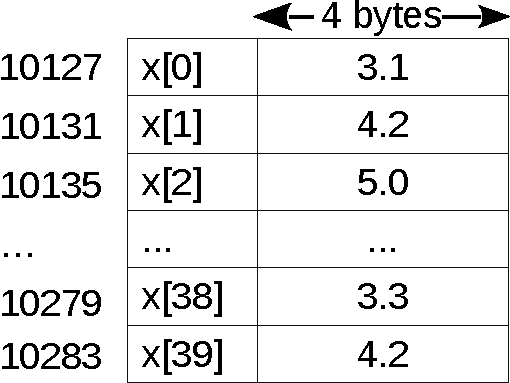
\includegraphics[width=0.90\linewidth]{figs/farray.pdf}
\end{figure}
\end{column}
\begin{column}{0.53\linewidth}
\begin{lstlisting}
#include <stdio.h>
int main()
{
   int a[10], b = 3;
   char c[10];
   printf("a: %d\n", sizeof(a));
   printf("b: %d\n", sizeof(b));
   printf("c: %d\n", sizeof(c));
   return 0;
}
\end{lstlisting}
\end{column}
\end{columns}
\vspace{0.1in}
\begin{itemize}
	\item {The system opens a continuous memory block for an array}
	\item {Actual size depends on both the type and length of an array}
\end{itemize}
\end{frame}

\begin{frame}[fragile]{1D Array: how array looks like (3)}
\begin{columns}
\begin{column}{0.53\linewidth}
\begin{lstlisting}
#include <stdio.h>
int main()
{
   int a[10], b = 3;
   char c[10];
   printf("a: %d\n", sizeof(a));
   printf("b: %d\n", sizeof(b));
   printf("c: %d\n", sizeof(c));
   return 0;
}
\end{lstlisting}
\end{column}
\begin{column}{0.4\linewidth}
[Output]
\begin{lstlisting}
a: 40
b: 4
c: 10
\end{lstlisting}
\end{column}
\end{columns}
\vspace{0.1in}
\begin{itemize}
	\item {Actual size depends on both the type and length of an array}
\end{itemize}
\end{frame}

\begin{frame}[fragile]{1D Array: initialization (1)}
\begin{itemize}
	\item {No initialization, what happens}
\end{itemize}
\vspace{-0.1in}
\begin{columns}
\begin{column}{0.33\linewidth}
[1: local]
\begin{lstlisting}[numbers=none]
#include <stdio.h>
int main()
{
 int a[10];
 int i = 0;
 for(;i < 10; i++)
 printf("%d ",a[i]);
 return 0;
}
\end{lstlisting}
\end{column}
\begin{column}{0.33\linewidth}
[2: static]
\begin{lstlisting}[numbers=none]
#include <stdio.h>
int main()
{
 static int a[10];
 int i = 0;
 for(;i<10; i++)
 printf("%d ",a[i]);
 return 0;
}
\end{lstlisting}
\end{column}
\begin{column}{0.33\linewidth}
[3: external]
\begin{lstlisting}[numbers=none]
#include <stdio.h>
extern a[10];
int main()
{
 int i = 0;
 for(; i<10; i++)
 printf("%d ",a[i]);
 return 0;
}
\end{lstlisting}
\end{column}
\end{columns}
\begin{enumerate}
	\item {Initialize to random numbers}
	\item {Initialize to zeros}
	\item {Initialize to zeros}
\end{enumerate}

\end{frame}

\begin{frame}[fragile]{1D Array: initialization (2)}
\begin{itemize}
	\item {Initializations as follows are \textcolor{green}{valid}}
\end{itemize}
\begin{columns}
\begin{column}{0.45\linewidth}
\begin{lstlisting}
#include <stdio.h>
int main()
{
   int a[10] = {3, 2, 5, 1};
   int i = 0;
   for(; i < 10; i++)
   printf("%d ",a[i]);
   return 0;
}
\end{lstlisting}
\end{column}
\begin{column}{0.45\linewidth}
\begin{lstlisting}
#include <stdio.h>
int main()
{
   int a[] = {3, 2, 5, 1};
   int i = 0;
   for(; i < 4; i++)
   printf("%d ",a[i]);
   return 0;
}
\end{lstlisting}
\end{column}
\end{columns}
\end{frame}

\begin{frame}[fragile]{1D Array: initialization (3)}
\begin{itemize}
	\item {Initializations as follows are \textcolor{red}{invalid}}
\end{itemize}
\begin{columns}
\begin{column}{0.43\linewidth}
\begin{lstlisting}
#include <stdio.h>
int main()
{
   int a[10];
   a[10] = {3, 2, 5, 1};
   int i = 0;
   for(; i < 10; i++)
   printf("%d ",a[i]);
   return 0;
}
\end{lstlisting}
\end{column}
\begin{column}{0.43\linewidth}
\begin{lstlisting}
#include <stdio.h>
int main()
{
   int a = {3, 2, 5, 1};
   int i = 0;
   for(; i < 4; i++)
   printf("%d ",a[i]);
   return 0;
}
\end{lstlisting}
\end{column}
\end{columns}
\end{frame}

\begin{frame}{1D Array Example1 (1)}
	\begin{itemize}
		\item {Given an array: a[10] = \{3, 21, 5, 8, 5,11, 22,14,9,51\}}
		\item {Flip the array to: \{51, 9, 14, 22, 11, 5, 8, 5, 21, 3\}}
	\end{itemize}
	\vspace{0.2in}
	\begin{center}
		\Large{5 minutes to think about the solution}
	\end{center}
\end{frame}

\begin{frame}{1D Array Example1 (2)}
	\begin{itemize}
		\item {Given an array: a[10] = \{3, 21, 5, 8, 5,11, 22,14,9,51\}}
		\item {Flip the array to: \{51, 9, 14, 22, 11, 5, 8, 5, 21, 3\}}
	\end{itemize}
	\begin{itemize}
		\item {The idea is that, we only need to swap two elements each time}
		\item {One for the header, one from the rear}
		\item {We do this for $\frac{10}{2}$ times}
	\end{itemize}
\end{frame}

\begin{frame}{1D Array Example1 (3)}
	\begin{itemize}
		\item {Given an array: a[10] = \{3, 21, 5, 8, 5,11, 22,14,9,51\}}
		\item {Flip the array to: \{51, 9, 14, 22, 11, 5, 8, 5, 21, 3\}}
	\end{itemize}
	\begin{enumerate}
		\item {For i from 0 to $\frac{N}{2}$ do}
		\item {~~~Exchange a[i] with a[N-i-1]}
		\item {End-for}
	\end{enumerate}
	\begin{itemize}
		\item {Let's do it, give you another 5 minutes ...}
	\end{itemize}
\end{frame}

\begin{frame}[fragile]{1D Array Example1 (4)}
	\begin{enumerate}
		\item {For i from 0 to $\frac{N}{2}$ do}
		\item {~~~Exchange a[i] with a[N-i-1]}
		\item {End-for}
	\end{enumerate}
\begin{lstlisting}[xleftmargin=0.08\linewidth,linewidth=0.9\linewidth]
#include <stdio.h>
int main()
{
   int a[10] ={3,21,5,8,5,11,22,14,9,51};
   int t = 0, i = 0;
   for(; i < 5; i++){
       t = a[i];
       a[i] = a[10-i-1];
       a[10-i-1] = t;
   }
   for(i = 0; i < 10; i++){
       printf("%d ", a[i]);
   }
   return 0;
}
\end{lstlisting}
\end{frame}

\begin{frame}{1D Array Example2 (1)}
	\begin{itemize}
		\item {Given an array: a[10] = \{21, 3, 5, 8, 5,11, 22,14,51,9\}}
		\item {Sort the array in ascending order: \{3, 5, 5, 8, 9, 11, 14, 21, 22, 51\}}
	\end{itemize}
	\vspace{0.2in}
	\begin{center}
		\Large{5 minutes to think about the solution...}
	\end{center}
\end{frame}

\begin{frame}{1D Array Example2 (2)}
	\begin{itemize}
		\item {Given an array: a[10] = \{21, 3, 5, 8, 5,11, 22,14,9,51\}}
		\item {Sort the array in ascending order: \{3, 5, 5, 8, 9, 11, 14, 21, 22, 51\}}
	\end{itemize}
	\begin{itemize}
		\item {The idea is bubble sort, which is a classic method for sorting}
		\item {Each time, we move the largest to the rear of the array}
		\item {Repeat this on sub-array for N times}
	\end{itemize}
\end{frame}

\begin{frame}{1D Array Example2 (3)}
\begin{figure}
	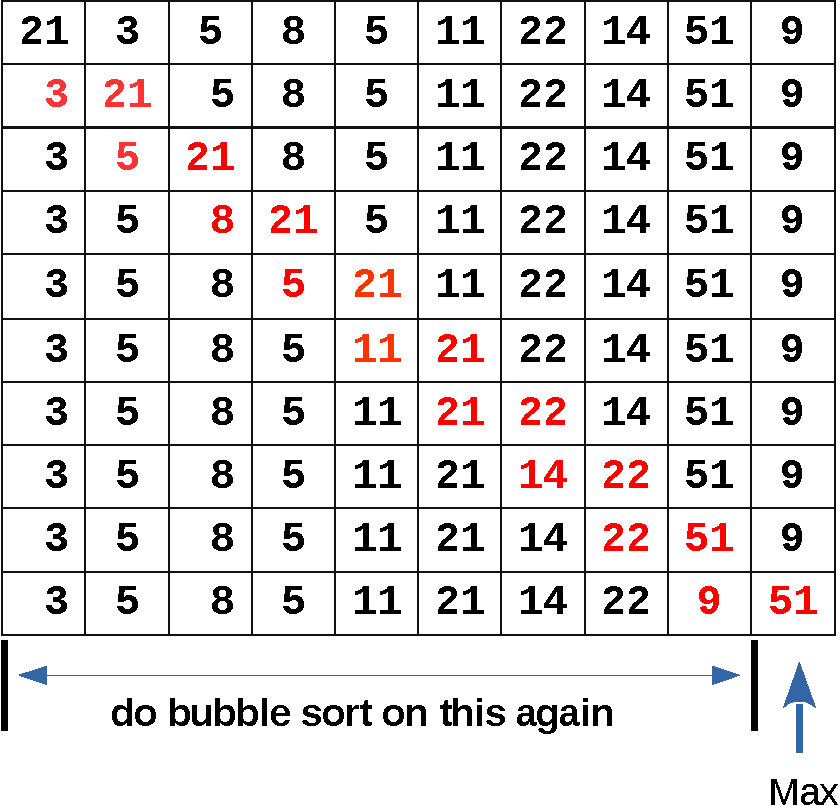
\includegraphics[width=0.55\linewidth]{figs/bubblesort.pdf}
	\caption{Demo of one round of bubble sort}
\end{figure}
\end{frame}

\begin{frame}{1D Array Example2 (4)}
\begin{itemize}
	\item {Let's now outline the procedure}
\end{itemize}
\begin{enumerate}
	\item {For i from 0 to N do}
	\item {~~For j from 0 to N-i do}
	\item {~~~~Check a[j] and a[j+1]}
	\item {~~~~If a[j] $>$ a[j+1]}
	\item {~~~~~swap them}
	\item {~~~~End-if}
	\item {~~End-for(j)}
	\item {End-for(i)}
\end{enumerate}
\end{frame}

\begin{frame}[fragile]{1D Array Example2 (5): the code}
\vspace{-0.1in}
\begin{lstlisting}[xleftmargin=0.08\linewidth,linewidth=0.9\linewidth]
#include <stdio.h>
int main()
{
   int a[10] = {3, 5, 5, 8, 9, 11, 14, 21, 22, 51};
   int i = 0, j = 0, t = 0;
   for(i = 0; i < 10; i++) {
      for(j = 0; j < (10-i-1); j++) {
          if(a[j] > a[j+1]) 
          {
             t = a[j];
             a[j] = a[j+1];
             a[j+1] = t;
          }//if(a[j])
      }//for(j)
   }//for(i)
   for(i = 0; i < 10; i++) {
      printf("%d ", a[i]);
   }   
   return 0;
}
\end{lstlisting}
\end{frame}

\subsection{2D Array}
\label{sec:2darry}
\begin{frame}<beamer>
    \frametitle{Outline}
    \tableofcontents[currentsection, currentsubsection]
\end{frame}

\begin{frame}[fragile]{Opening Discussion: 2D Array}
	\begin{itemize}
		\item {Continue with the opening example in the last section}
		\item {In your class, you might have several courses for each student}
		\item {So we need several 1D arrays}
		\item {Alternatively, we can use a 2D array}
	\end{itemize}
\begin{columns}
\begin{column}{0.4\linewidth}
\begin{lstlisting}
int main()
{
    float math[40];
    float c[40];
    float phis[40];
    float bio[40];
    ...
}
\end{lstlisting}
\end{column}
\begin{column}{0.4\linewidth}
\begin{lstlisting}
int main()
{
    float courses[40][4];
    ...
}
\end{lstlisting}
\end{column}
\end{columns}
\end{frame}

\begin{frame}[fragile]{2D Array: declaration}
\begin{center}
	\LARGE{
	 \textcolor{blue}{type} \textcolor{red}{arrayName}[\textbf{row}][\textbf{column}];
	}
\end{center}

	\begin{itemize}
		\item {Similar as 1D array, \textcolor{blue}{type} is required}
		\item {``\textcolor{red}{arrayName}'' should be unique}
		\item {``row'' and ``column'' should be constant expressions}
	\end{itemize}
\begin{lstlisting}
int main()
{
   float a[40][4]; //there 40 rows and 4 columns in each row
   a[3][2] = 3.14;
   return 0;
}
\end{lstlisting}
\end{frame}

\begin{frame}[fragile]{2D Array: initialization (1)}
\begin{lstlisting}
int main()
{
   float a[3][4] = {{1,3,1,1},{1,2,1,3},{1,12,1,2}};
   return 0;
}
\end{lstlisting}
\begin{itemize}
	\item {Following way is also \textcolor{green}{valid}}
\end{itemize}
\begin{lstlisting}
int main()
{
   float a[3][4] = {1,3,1,1,1,2,1,3,1,12,1,2};
   return 0;
}
\end{lstlisting}
\end{frame}

\begin{frame}[fragile]{2D Array: initialization (2)}
\begin{lstlisting}
int main()
{
   float a[][4] = {{1,3,1,1},{1,2,1,3},{1,12,1,2}};
   return 0;
}
\end{lstlisting}
\begin{itemize}
	\item {Following way is also \textcolor{green}{valid}, $row=\lceil\frac{N}{4}\rceil$}
\end{itemize}
\begin{lstlisting}
int main()
{
   float a[][4] = {1,3,1,1,1,2,1,3,1,12,1,2};
   return 0;
}
\end{lstlisting}
\begin{itemize}
	\item {If no initialization, set to \textcolor{red}{0} by default}
\end{itemize}
\end{frame}

\begin{frame}[fragile]{2D Array: initialization (3)}
\begin{lstlisting}
int main()
{
   float a[][4] = {{1,3,1,1},{1,2,1,3},{1,12,1,2}};
   return 0;
}
\end{lstlisting}
\begin{itemize}
	\item {Following way is also \textcolor{red}{invalid}}
\end{itemize}
\begin{lstlisting}
int main()
{
   float a[4][] = {1,3,1,1,1,2,1,3,1,12,1,2};
   return 0;
}
\end{lstlisting}
\begin{itemize}
	\item {It is organized in row major order}
\end{itemize}
\end{frame}

\begin{frame}[fragile]{2D Array: how it looks like}
\begin{figure}
	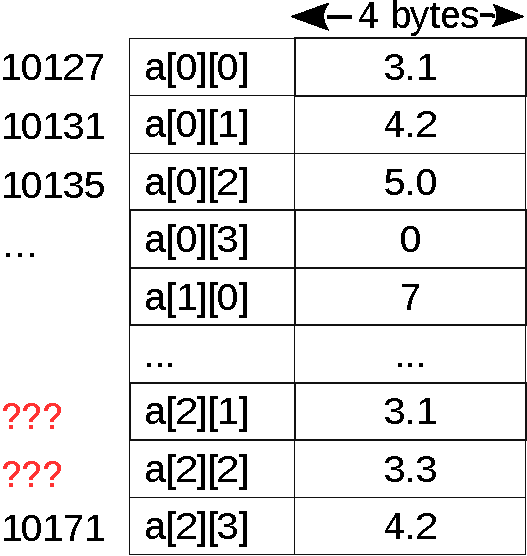
\includegraphics[width=0.4\linewidth]{figs/farray2d.pdf}
\end{figure}
\begin{itemize}
	\item {$3$(row)${\times}4$(column)${\times}4$ bytes}
\end{itemize}
\end{frame}

\begin{frame}[fragile]{2D Array: visit element of the array}
\begin{lstlisting}[xleftmargin=0.08\linewidth, linewidth=0.85\linewidth]
int main()
{
   float a[][4] = {1,3,1,1,1,2,1,3,1,12,1,2};
   int i = 0, j = 0;
   for(i = 0; i < 3; i++)
   {
      for(j = 0; j < 4; j++)
      {
          printf("%f ", a[i][j]);
      }
      printf("\n");
   }
   return 0;
}
\end{lstlisting}
\end{frame}
\section{Strings}
\label{sec:str}
\begin{frame}<beamer>
    \frametitle{Outline}
    \tableofcontents[currentsection]
\end{frame}

\begin{frame}[fragile]{Opening discussion}
	\begin{itemize}
		\item {Now, we are going to discuss a special kind of array}
		\item {Array of chars, we give it a new name \textbf{string}}
		\item {Different from integer array, empty elements are set to `$\setminus$0'}
	\end{itemize}
	\begin{columns}
	\begin{column}{0.47\linewidth}
	\begin{lstlisting}
#include <stdio.h>
int main()
{
    char hi[8] ={'h','e','l','l','o'};
    int i = 0;
    for(i < 8; i++)
    {
       printf("%c", hi[i]);
    }
    return 0;
}
	[Output: hello   ]
	\end{lstlisting}
	\end{column}
	\begin{column}{0.47\linewidth}
	\begin{lstlisting}
#include <stdio.h>
int main()
{
    char hi[8] ={'h','e','l','l','o'};
    int i = 0;
    printf("%s", hi);
    return 0;
}
	[Output: hello]
	\end{lstlisting}
	\end{column}
	\end{columns}
\end{frame}

\begin{frame}[fragile]{String: definition and initialization}
\begin{itemize}
	\item {First of all, it is an array}
	\item {We can initialize it as an array}
\end{itemize}
\begin{lstlisting}
#include <stdio.h>
int main()
{
   char ch[6] = {'H','e','l','l','o','\0'};
   char ch[]  = {'H','e','l','l','o','\0'};
   /*we have 6 chars there*/
   char ch[6] = {'H','e','l','l','o'}; 
   /*'\0' is automatically appended **/
   char ch[6] = {"Hello"};
   char ch[6] = "Hello";
   char ch[]  = "Hello";
   return 0;
}
\end{lstlisting}
\end{frame}

\begin{frame}[fragile]{String Operation: strcpy}
\begin{itemize}
	\item {Copy one string to another}
	\item {strcpy(destine, source)}
\end{itemize}
\begin{columns}
\begin{column}{0.45\linewidth}
\begin{lstlisting}
#include <stdio.h>
#include <string.h>
int main()
{
   char ch[10];
   strcpy(ch, "hi");
   printf("%s\n", ch);
   strcpy(ch, "ha");
   printf("%s\n", ch);
   return 0;
}
\end{lstlisting}
\end{column}
\begin{column}{0.45\linewidth}
[Output:]
\begin{lstlisting}
hi
ha
\end{lstlisting}
\end{column}
\end{columns}
\end{frame}


\begin{frame}[fragile]{String Operation: strcmp (1)}
\begin{itemize}
	\item {\textcolor{red}{C}o\textcolor{red}{mp}are whether two strings are equal or not}
\end{itemize}
\begin{columns}
\begin{column}{0.85\linewidth}
\begin{lstlisting}[xleftmargin=0.05\linewidth, linewidth=0.94\linewidth]
#include <stdio.h>
#include <string.h>
int main()
{
  char ch1[10], ch2[10];
  strcpy(ch1, "hi");
  strcpy(ch2, "ha");
  if(strcmp(ch1, ch2) == 1){
      printf("ch1 > ch2\n");
  }else if(strcmp(ch1,ch2)==-1)
  {
      printf("ch1 < ch2\n");
  }
  else if(strcmp(ch1,ch2)==0){
      printf("identical");
  }
}
\end{lstlisting}
\end{column}
\begin{column}{0.15\linewidth}
[Output]\\
ch1 $>$ ch2
\end{column}
\end{columns}

\end{frame}


\begin{frame}[fragile]{String Operation: strcmp (2)}
\vspace{-0.10in}
\begin{itemize}
	\item {\textcolor{red}{C}o\textcolor{red}{mp}are whether two strings are equal or not}
\end{itemize}
\vspace{-0.10in}
\begin{columns}
\begin{column}{0.85\linewidth}
\begin{lstlisting}[xleftmargin=0.05\linewidth, linewidth=0.94\linewidth]
#include <stdio.h>
#include <string.h>
int main()
{
  char ch1[10], ch2[10];
  strcpy(ch1, "he");
  strcpy(ch2, "we");
  if(strcmp(ch1, ch2) == 1)
  {
      printf("ch1 > ch2\n");
  }else if(strcmp(ch1,ch2)==-1)
  {
      printf("ch1 < ch2\n");
  }
  else if(strcmp(ch1,ch2)==0)
  {
      printf("identical");
  }
}
\end{lstlisting}
\end{column}
\begin{column}{0.15\linewidth}
[Output]\\
ch1 $<$ ch2
\end{column}
\end{columns}
\end{frame}

\begin{frame}[fragile]{String Operation: strcmp (3)}
\begin{itemize}
	\item {\textcolor{red}{C}o\textcolor{red}{mp}are whether two strings are equal or not}
\end{itemize}
\vspace{-0.15in}
\begin{columns}
\begin{column}{0.85\linewidth}
\begin{lstlisting}[xleftmargin=0.05\linewidth, linewidth=0.94\linewidth]
#include <stdio.h>
#include <string.h>
int main()
{
  char ch1[10], ch2[10];
  strcpy(ch1, "hi");
  strcpy(ch2, "hi");
  if(strcmp(ch1, ch2)!=0)
  {
      printf("different");
  }
  else if(strcmp(ch1, ch2)==0)
  {
      printf("identical");
  }
  return 0;
}
\end{lstlisting}
\end{column}
\begin{column}{0.15\linewidth}
[Output]\\
identical
\end{column}
\end{columns}
\end{frame}

\begin{frame}[fragile]{String Operation: strlen (1)}
\begin{itemize}
	\item {Calculate the \textcolor{red}{len}gth of the string}
	\item {Pass the string until it encounters `$\setminus$0'}
\end{itemize}
\begin{columns}
\begin{column}{0.5\linewidth}
\begin{lstlisting}
#include <stdio.h>
#include <string.h>
int main()
{
   char a[20] = "hello";
   int l = strlen(a);
   printf("length is: %d", l);
   return 0;
}
\end{lstlisting}
[length is: 5]
\end{column}
\begin{column}{0.5\linewidth}
\begin{lstlisting}
#include <stdio.h>
#include <string.h>
int main()
{
   char a[20] = "hello world";
   int l = strlen(a);
   printf("length is: %d", l);
   return 0;
}
\end{lstlisting}
[length is: 11]
\end{column}
\end{columns}
\end{frame}

\begin{frame}[fragile]{String Operation: strlen (2)}
\begin{itemize}
	\item {Calculate the \textcolor{red}{len}gth of the string}
	\item {Pass the string until it encounters `$\setminus$0'}
\end{itemize}
\begin{columns}
\begin{column}{0.5\linewidth}
\begin{lstlisting}
#include <stdio.h>
#include <string.h>
int main()
{
   char a[20] = "hello world";
   int l = strlen(a);
   printf("length is: %d", l);
   return 0;
}
\end{lstlisting}
[length is: 11]
\end{column}
\begin{column}{0.5\linewidth}
\begin{lstlisting}
#include <stdio.h>
#include <string.h>
int main()
{
   char a[20]="hello\0world";
   int l = strlen(a);
   printf("length is: %d", l);
   return 0;
}
\end{lstlisting}
[length is: 5]
\end{column}
\end{columns}
\end{frame}


\begin{frame}[fragile]{String Operation: strcat}
\begin{itemize}
	\item {Con\textcolor{red}{cat}enate two strings into one}
\end{itemize}
\begin{columns}
\begin{column}{0.45\linewidth}
\begin{lstlisting}
#include <stdio.h>
#include <string.h>
int main()
{
   char a[20] = "hello ";
   char b[10] = "world";
   printf("a=%s\n", a);
   printf("b=%s\n", b);
   strcat(a, b);
   printf("a=%s\n", a);
   return 0;
}
\end{lstlisting}
\end{column}
\begin{column}{0.45\linewidth}
\begin{lstlisting}
hello
world
hello world
\end{lstlisting}
\end{column}
\end{columns}
\end{frame}

\begin{frame}[fragile]{Summary over string and char array}
\begin{itemize}
	\item {Array of chars could be used as string, `$\setminus$0' should be appended at the end}
	\item {One more byte should be reserved for `$\setminus$0'}
	\item {String can be used as an array of chars}
	\item {Functions such as ``strcpy'', ``strlen'', ``strcat'' etc require string input}
\end{itemize}

\begin{table}
\begin{center}
	\begin{tabular}{|l|l|} \hline
	 Usage & Comments \\ \hline
	\multirow{2}{*}{\textcolor{blue}{strcpy}(str1, str2)} & Copy ``str2'' to ``str1'', the content \\ & of ``str1'' will be overwriten \\ \hline
	 \textcolor{blue}{strlen}(str1) & Calculate the number of characters before `$\setminus$0' \\ \hline
	\textcolor{blue}{strcat}(str1, str2) & Concatenate ``str2'' to ``str1'' and save to ``str1'' \\ \hline
	\multirow{2}{*}{\textcolor{blue}{strcmp}(str1, str2)} & Compare two strings, \\ & returns -1, 1 or 0 if they are identical \\ \hline
	\end{tabular}
\end{center}
\end{table}

\end{frame}
\section{}
\end{document}
